\newcommand{\DoNotLoadEpstopdf}{}
\documentclass[tikz,border=7pt]{standalone}
\usepackage{amsmath,amssymb}
\usetikzlibrary{arrows.meta,calc}
\definecolor{shared}{RGB}{170,48,60}
\definecolor{local}{RGB}{0,0,0}
\definecolor{line}{RGB}{0,0,0}
\tikzset{
 axis/.style={line width=.9pt,line,-{Latex[length=2mm,width=1.4mm]}},
 badge/.style={circle,draw,line width=.8pt,minimum size=5mm,inner sep=0pt,font=\small,fill=white},
 title/.style={font=\normalsize,text=local},
 eq/.style={font=\small,text=local}
}
\newcommand{\components}[3]{
 \draw[axis] (0,0)--(0,1.65);
 \draw[axis] (0,0)--(1.65,0);
 \node[badge,draw=#1,text=#1] at (-.45,1.32){1};
 \draw[#2,line width=.8pt,{Latex[length=1.2mm]}-{Latex[length=1.2mm]}]
 (0,.72) to[bend left=40] (.72,0);
 \node[badge,draw=#2,text=#2] at (.73,.79){2};
 \node[badge,draw=#3,text=#3] at (1.3,-.46){3};
}
\begin{document}
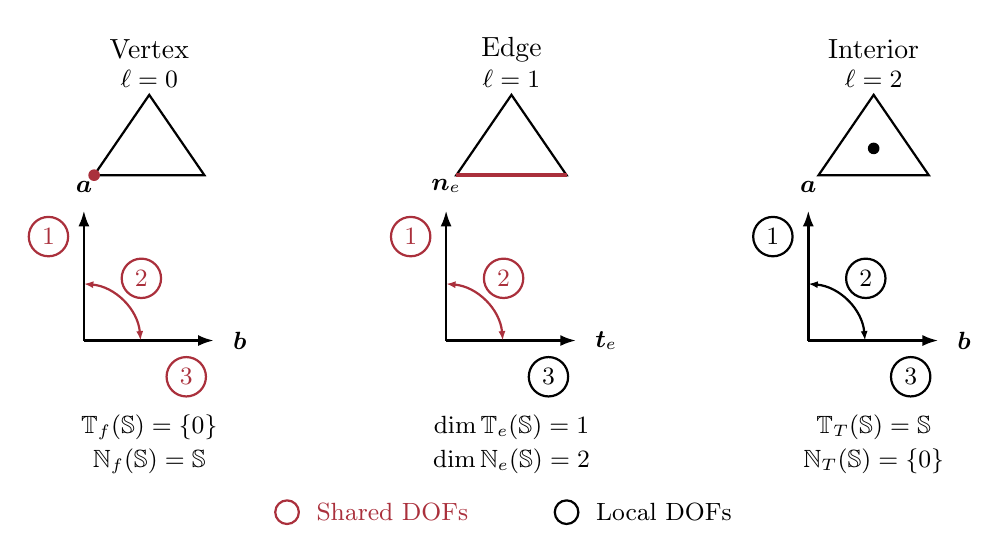
\begin{tikzpicture}[x=1cm,y=1cm]
% Three entity columns without decorative panels. Numbers retain the original tensor-component meanings.
\foreach \x/\name/\dim in {0/Vertex/0,4.6/Edge/1,9.2/Interior/2}{
 \node[title] at (\x+2.15,5.25){\name};
 \node[text=line,font=\small] at (\x+2.15,4.87){$\ell=\dim$};
 \begin{scope}[shift={(\x+1.45,3.65)}]
   \coordinate (A) at (0,0);\coordinate (B) at (1.4,0);\coordinate (C) at (.7,1.02);
   \draw[line,line width=.8pt] (A)--(B)--(C)--cycle;
 \end{scope}
}
% Highlight the entity represented by each panel.
\fill[shared] (1.45,3.65) circle (2.1pt);
\draw[shared,line width=1.6pt] (6.05,3.65)--(7.45,3.65);
\fill[local] (11.35,3.99) circle (2.1pt);
\begin{scope}[shift={(1.32,1.55)}]
 \components{shared}{shared}{shared}
 \node[text=line,font=\small,anchor=south] at (0,1.75){$\boldsymbol a$};
 \node[text=line,font=\small,anchor=west] at (1.77,0){$\boldsymbol b$};
\end{scope}
\begin{scope}[shift={(5.92,1.55)}]
 \components{shared}{shared}{local}
 \node[text=line,font=\small,anchor=south] at (0,1.75){$\boldsymbol n_e$};
 \node[text=line,font=\small,anchor=west] at (1.77,0){$\boldsymbol t_e$};
\end{scope}
\begin{scope}[shift={(10.52,1.55)}]
 \components{local}{local}{local}
 \node[text=line,font=\small,anchor=south] at (0,1.75){$\boldsymbol a$};
 \node[text=line,font=\small,anchor=west] at (1.77,0){$\boldsymbol b$};
\end{scope}
\node[eq] at (2.15,.45){$\mathbb T_f(\mathbb S)=\{0\}$};
\node[eq] at (2.15,.02){$\mathbb N_f(\mathbb S)=\mathbb S$};
\node[eq] at (6.75,.45){$\dim\mathbb T_e(\mathbb S)=1$};
\node[eq] at (6.75,.02){$\dim\mathbb N_e(\mathbb S)=2$};
\node[eq] at (11.35,.45){$\mathbb T_T(\mathbb S)=\mathbb S$};
\node[eq] at (11.35,.02){$\mathbb N_T(\mathbb S)=\{0\}$};
% Color key; tensor-component definitions are given in the caption.
\node[draw=shared,line width=.8pt,circle,minimum size=3mm,inner sep=0pt] at (3.9,-.63){};
\node[anchor=west,font=\small,text=shared] at (4.15,-.63){Shared DOFs};
\node[draw=local,line width=.8pt,circle,minimum size=3mm,inner sep=0pt] at (7.45,-.63){};
\node[anchor=west,font=\small,text=local] at (7.7,-.63){Local DOFs};
\end{tikzpicture}
\end{document}
